\documentclass{article}

\usepackage[utf8]{inputenc}
\usepackage[T1]{fontenc}
\usepackage{fourier}
%\usepackage[latin1]{inputenc}
\usepackage[spanish]{babel}

\usepackage[thinlines]{easytable}
\usepackage{diagbox}
\usepackage{multirow}


\usepackage[protrusion=true,expansion=true]{microtype}	
\usepackage{amsmath,amsfonts,amsthm} % Math packages
\usepackage{amssymb}
\usepackage[pdftex]{graphicx}	
\usepackage{url}
\usepackage{tikz}
\usepackage{setspace}
\usepackage{import}
\usepackage{float}
\usepackage{graphicx}
\pagenumbering{arabic}
%margenes 
\usepackage{geometry}
 \geometry{
 a4paper,
 left=19mm,
 right=19mm,
 top=19mm,
 bottom=42mm,
 }

% %%% Custom sectioning
\usepackage{sectsty}
%\allsectionsfont{\normalfont \scshape}


%%% Custom headers/footers (fancyhdr package)
\usepackage{fancyhdr}
\pagestyle{fancyplain}
\fancyhead{}											% No page header
\fancyfoot[L]{}											% Empty 
\fancyfoot[C]{}											% Empty
\fancyfoot[R]{\thepage}									% Pagenumbering
\renewcommand{\headrulewidth}{0pt}			% Remove header underlines
\renewcommand{\footrulewidth}{0pt}				% Remove footer underlines
\setlength{\headheight}{13.6pt}


%%% Equation and float numbering
\numberwithin{equation}{section}		% Equationnumbering: section.eq#
\numberwithin{figure}{section}			% Figurenumbering: section.fig#
\numberwithin{table}{section}				% Tablenumbering: section.tab#


%%% Maketitle metadata
\newcommand{\horrule}[1]{\rule{\linewidth}{#1}} 	% Horizontal rule

\begin{document}
\onehalfspacing

\begin{titlepage}
    
\newcommand{\HRule}{\rule{\linewidth}{0.5mm}} % Defines a new command for the horizontal lines, change thickness here
    
\center % Center everything on the page
     
%----------------------------------------------------------------------------------------
%	HEADING SECTIONS
%----------------------------------------------------------------------------------------
    
\textsc{\LARGE Instituto Tecnológico de Buenos Aires}\\[2cm] % Name of your university/college
\textsc{\Large 22.42 Laboratorio de Electrónica}\\[1.5cm] % Major heading such as course name
\textsc{\large Trabajo Práctico N° 2}\\[0.5cm] % Minor heading such as course title
    
%----------------------------------------------------------------------------------------
%	TITLE SECTION
%----------------------------------------------------------------------------------------
    
\HRule \\[0.5cm]
{ \huge \bfseries Osciloscopios/ Analizador de Impedancias/ \\Circuitos RLC}\\[0.4cm] % Title of your document
\HRule \\[2cm]
     
%----------------------------------------------------------------------------------------
%	AUTHOR SECTION
%----------------------------------------------------------------------------------------
    
\begin{minipage}{0.4\textwidth}
\begin{flushleft} \large
\emph{Grupo 5:}\\		%names
[.3cm]
Nicolás \textsc{De León}\\
Leg. 57232\\ 
[.3cm]
Tomás \textsc{Vigón}\\
Leg. 57327\\ 
[.3cm]
Benjamín \textsc{Lin}\\
Leg. 57242 \\ 
[.3cm]
Lucero Guadalupe \textsc{Fernandez}\\
Leg. 57485\\ 
[.3cm]
\end{flushleft}
\end{minipage}
~
\begin{minipage}{0.4\textwidth}
\begin{flushright} \large
\emph{Profesor:} \\
[.3cm]
Pablo  \textsc{Cossutta}\\ % Supervisor's Name
Alejandra \textsc{Weill} \\% Supervisor's Name
Matías  \textsc{Salvati} % Supervisor's Name
\end{flushright}
\end{minipage}\\[2cm]
    
%----------------------------------------------------------------------------------------
%	DATE SECTION
%----------------------------------------------------------------------------------------
    
\vfill
{\large Entregado: 25 de Septiembre de 2018}\\[2cm]
    
\vfill 
    
\end{titlepage}

\section{Análisis de circuito RC}

Se armó el circuito de la figura inferior con los valores nominales de $R=3.9k\Omega$ y $C=1.8nF$.
\begin{figure}[h!]
\centering
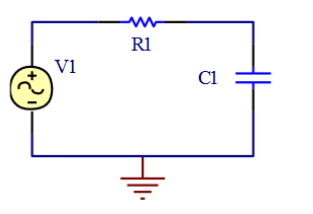
\includegraphics[scale=0.5]{rcCircuito.png}
\caption{Circuito RC armado.}
\label{fig:RC}
\end{figure}

\subsection{Cálculo de Frecuencia de Corte}

La frecuencia de corte es aquella en la que la salida $V_{out}$ atenúa la entrada $V_{in}$ en $-3dB$ y la primera desfasa a la segunda en $45^o$; de esta manera
se buscó experimentalmente su respectiva frecuencia de corte que resultó ser $f_{cmedido}=21.8kHz$. Se tuvo en cuenta la resistencia interna
del generador ($50\Omega$), y se la sumó a la $R_{teorica}$ .

A continuación, sabiendo que $C_{cal}\text{=}\frac{1}{2\pi fR}$ se completó la siguiente tabla:

\begin{table}[!htb]
\centering
\begin{tabular}{|c|c|c|c|c|c|}
\hline 
$|V_{in}|[V]$ & $|V_{out}|[V]$ & $R[k\Omega]$ & $C_{calculado}[nF]$ & $C_{medido}[nF]$ & $Error\%$\\
\hline 
\hline 
4.97 & 3.46 & 3.95 & 1.775 & 1.848 & 3.95\\
\hline 
4.97 & 3.46 & 3.93 & 1.784 & 1.848 & 3.46\\
\hline 
\end{tabular}
\caption{Tensiones y valores de componentes del circuito.}
\end{table}

\subsection{Medición de ángulo de fase entre I y $V_C$}

Para el cálculo de la corriente se utilizó $I=\frac{V_{R}}{R}$, asumiendo que la tensión y la corriente de la resistencia estaban en fase. 
Luego con el uso de la opción math del osciloscopio, se restó la caída en el capacitor a la tensión de entrada y se midieron las fases y amplitudes de las mismas, siendo la resultante de la resta $V_R$. Una vez que se obtuvo, se la dividió por el valor de la resistencia, obteniendo así, el valor vectorial de la corriente.
De esta manera se obtuvo que $|V_{R}|=3.51V$ y $|V_{c}|=3.48V$.

\begin{figure}[H]
\centering

\includegraphics[scale=0.5]{1-2.png}
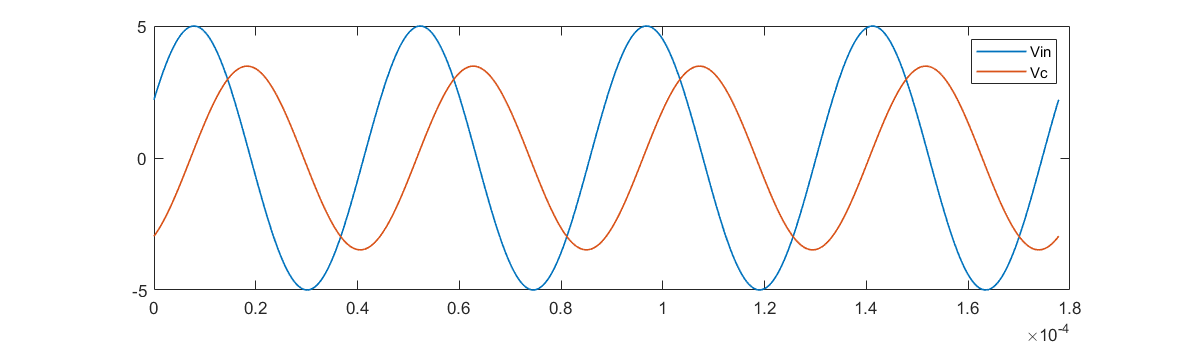
\includegraphics[scale=0.5]{1-2b.png}
\caption{Diagrama fasorial y representación de las señales VR y VC.}
\label{diagfasorial}
\end{figure}


De la figura \ref{diagfasorial} observamos que la corriente se adelanta a la tensión del capacitor $90^{o}$. Ademas, la suma fasorial de $V_R$ y $V_C$ es de 4.97V en vez de los 5V, esto puede ser por la resistencia del generador que aún siendo pequeña genera una caída de tensión en el circuito.

\subsection{Cálculo analítico de la función transferencia}

Teniendo en cuenta la fiugra \ref{RC}; con $V_{out}$ la tensión del capacitor y $V_{in}$ como la tensión de entrada que fue una senoidal de $5~V_{pp}$, se halló analíticamente la función transferencia planteando un divisor resistivo, que resultó ser:

\begin{center}
\begin{equation}
\label{transf}
H(s)=\frac{1}{sRC+1}
\end{equation}
\end{center}

siendo $s=j\omega$ y $R=R_{medida} + R_{generador}$.

La frecuencia de corte resulta ser el polo de la función, es decir, cuando 
$\omega_c=\frac{1}{RC}$. Entonces, teniendo en cuenta que $\omega=2\pi f$, se deduce que la frecuencia de corte es $f_{ccalculado}=22.75kHz$. 
Se puede ver que la función obtenida es un pasabajos con un polo simple en $\frac{1}{2\pi RC}$.
Se diagramó el Bode de magnitud y fase, que se muestra a continuación.

\begin{figure}[H]
\centering
\begin{minipage}{.5\textwidth}
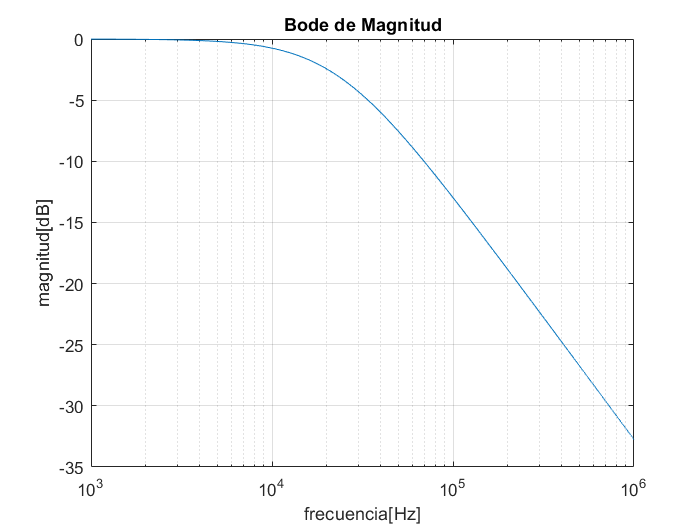
\includegraphics[scale=0.45]{1-3a.png}
\end{minipage}%
\begin{minipage}{.5\textwidth}
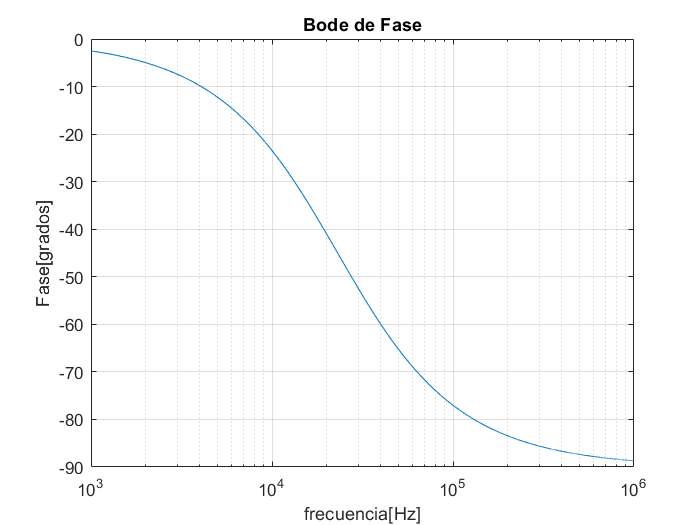
\includegraphics[scale=0.45]{1-3b.png}
\end{minipage}
\caption{Bode de magnitud y fase para los valores medidos de R y C.}
\label{diagbodemedido}
\end{figure}


En la figura \ref{diagbodemedido} puede verse que la frecuencia en la que la ganancia del circuito es $-3dB$ y el desfase es de $45^o$ es la frecuencia de corte, que ronda los 22.7kHz.

\subsection{Función transferencia a distintas frecuencias}

Se midieron valores de tensión y fase a distintas frecuencias entre 10Hz y 1MHz, completando la siguiente tabla. Donde el ángulo $\varphi_1$ fue medido en el modo $\Delta t$ del osciloscopio; y el ángulo $\varphi_2$, en el modo XY del osciloscopio.
//VALOR DE TENSION? 
La diferencia entre ambos $\varphi$ se debe a errores de apreciación al medir y de cálculo al realizar $\arcsin(\frac{\Delta X}{\Delta Y})$, siendo $\Delta X$ el ancho mínimo entre 2 extremos de la elipse y $\Delta Y$ el ancho máximo entre dos de ellos. 

\label{tablabode}

\subsection{Bode teórico y empírico}
Se graficó lo obtenido de la tabla \ref{tablabode} y se lo superpuso con el diagrama de Bode teórico de la función transferencia (ecuación \ref{transf}).

\begin{figure}[H]
\centering
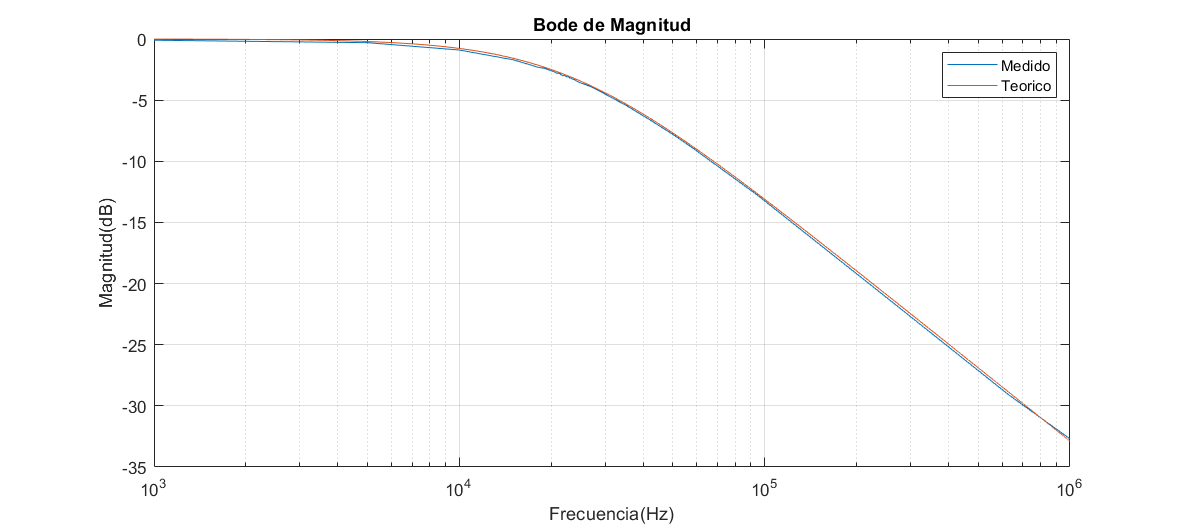
\includegraphics[scale=0.4]{1-4a.png}
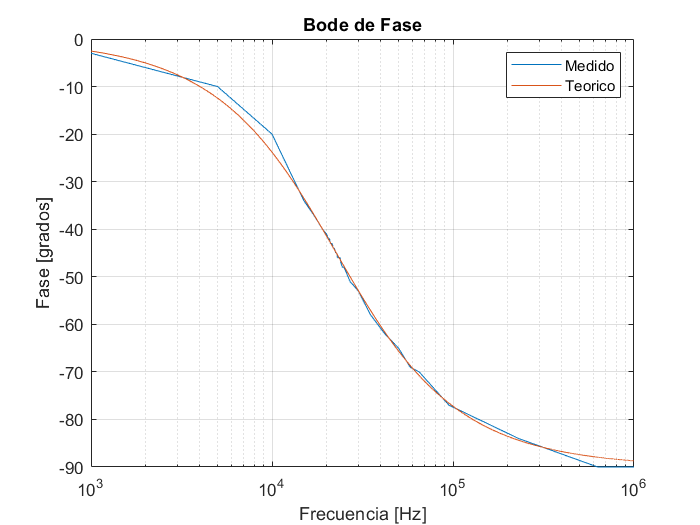
\includegraphics[scale=0.5]{1-4b.png}
\caption{Bode de magnitud y fase medido y teórico.}
\label{diagbode}
\end{figure}

Se puede observar que para el diagrama de amplitud las mediciones a distintas frecuencias se corresponden a lo calculado teóricamente. En el diagrama de fase, las variaciones se deben a errores de medición y en el rango de frecuencias altas, donde la señal es atenuada, se encuentra un mayor error ya que el ruido se hace comparable con la magnitud de la señal.

\subsection{Respuesta al escalón}

Se excitó al circuito con una señal cuadrada de $5~V_{pp}$ en un rango de frecuencias entre $500Hz$ y $500kHz$. Se destacaron las frecuencias $1kHz$, $15kHz$ y $200kHz$. Las mismas se muestran a continuación.

\begin{figure}[H]
\centering
\subfloat[Frecuencia 1kHz.]{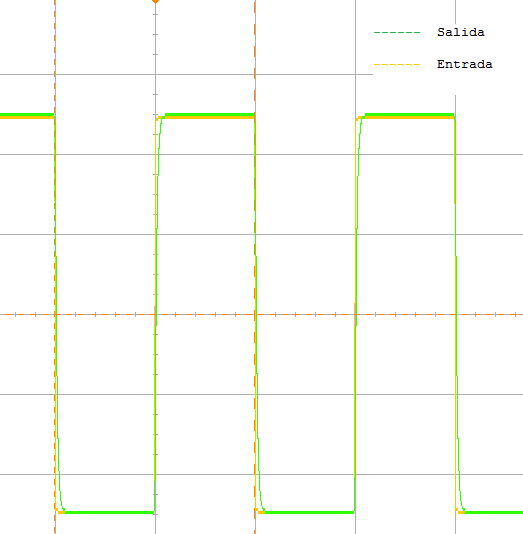
\includegraphics[scale=0.35]{1ka.png} }%
\qquad
\subfloat[Frecuencia 15kHz.]{{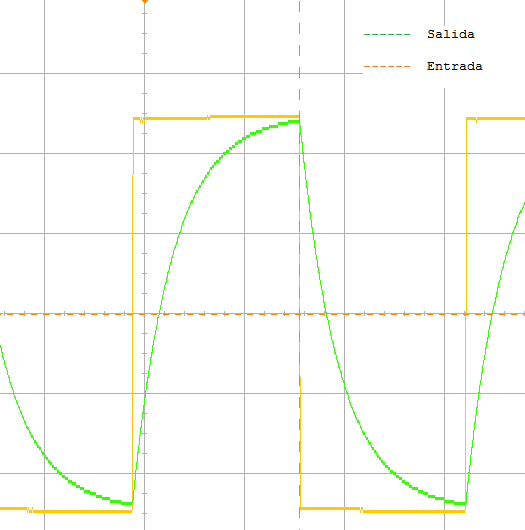
\includegraphics[scale=0.35]{15ka.png} }}%
\qquad
\subfloat[Frecuencia 200kHz.]{{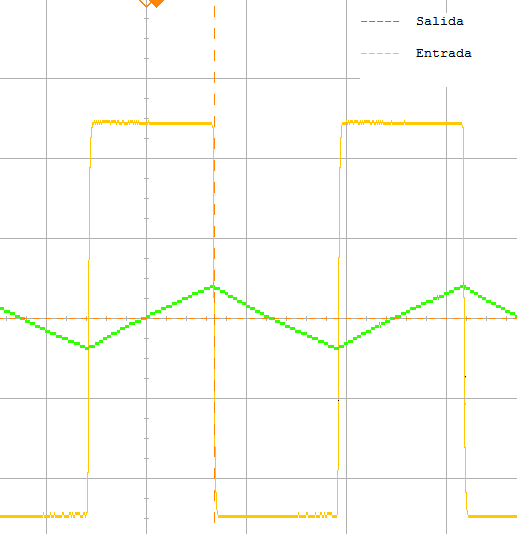
\includegraphics[scale=0.35]{200ka.png} }}%
\caption{Respuesta al escalón.}
\label{diagbodemedido}
\end{figure}

Si antitransformamos la función transferencia para obtener la respuesta en el tiempo, ésta resulta:
\begin{center}
\begin{equation}
\label{transf}
h(t)=\frac{e^{\frac{-t}{RC}}}{RC}
\end{equation}
\end{center}

Su respectiva respuesta al escalón será:
\begin{center}
\begin{equation}
\label{transf}
\widetilde{h}(t)=1 - e^{-\frac{t}{\tau}}
\end{equation}
\end{center}

con $\tau=RC$.
Cuando la frecuencia es de $1kHz$; como se ve en la figura \ref{diagbodemedido} $(a)$, debido a la baja frecuencia, el circuito logra llegar a un estado estacionario en lo que dura el período de la excitación cuadrada. Esto se debe a que el tiempo característico del circuito $\tau=RC=6.84\mu s$, que es mucho menor al período de la señal de entrada $T=1ms$.
Al excitar el circuito con una frecuencia de $15kHz$, cuyo período es de $ T\approx 66.67\mu s$, que ya es comparable con el tiempo característico del circuito, se llega a apreciar el estado transitorio del mismo. Esto se puede apreciar en la figura \ref{diagbodemedido} $(b)$.
En el último caso, en la figura \ref{diagbodemedido} $(c)$, con una frecuencia de $200kHz$, no se llega al estado estacionario, sino que se observa una fracción del transitorio, que se debe a que el período de la excitación cuadrada se vuelve menor al tiempo característico del circuito $(T\approx 5\mu s)$. Lo que se está viendo es la pendiente de la exponencial, que se asemeja con una recta.
Se puede notar que a frecuencias mucho mayores a su frecuencia de corte, la función transferencia puede aproximarse a $H(s)=\frac{1}{sRC}$, que es la transferencia de un circuito integrador. De este análisis se deriva, que a altas frecuencias el circuito integra.

\subsection{Respuesta en frecuencia de VR}




\textbf{1.8}
//1.7
//imagenes 1.8

\textbf{1.9 Conclusiones}

<<<<<<< HEAD
De esto se concluye, de ahí que a altas frecuencias el circuito integra.

\section{parte2}
=======


\section{Analisis Circuito CR}

Se armó el circuito de la figura inferior con los componentes anteriores.

\begin{figure}[h!]
\centering
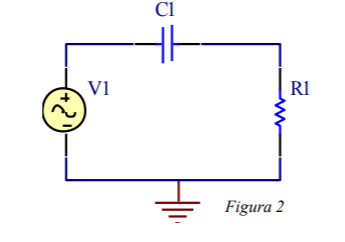
\includegraphics[scale=0.5]{crCircuito.png}
\caption{Circuito CR armado.}
\label{fig:CR}
\end{figure}


\subsection{Funcion de Transferencia}

Como la funcion de transferencia en este circuito es $H(s) = \frac{V_R(s)}{V_1}$ y conciderenado la resistencia del generador, la funcion de transferencia resulta ser:
$$H(s) = \frac{sCR}{\left(R+R_{gen}\right)Cs+1}$$
Por lo que notamos que a mayor frecuencia la tension del $V_R$ aumenta a mayor frecuencia, por lo que tiene caractestica de un filtro pasa alto. Es posible visualisar este comportamiento en el siguiente diagrama de Bode:

\begin{figure}[h!]
\centering
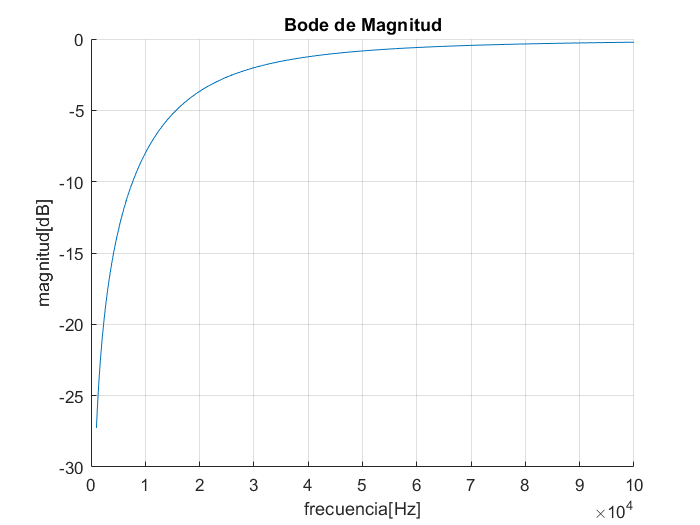
\includegraphics[scale=0.5]{2teomag.png}
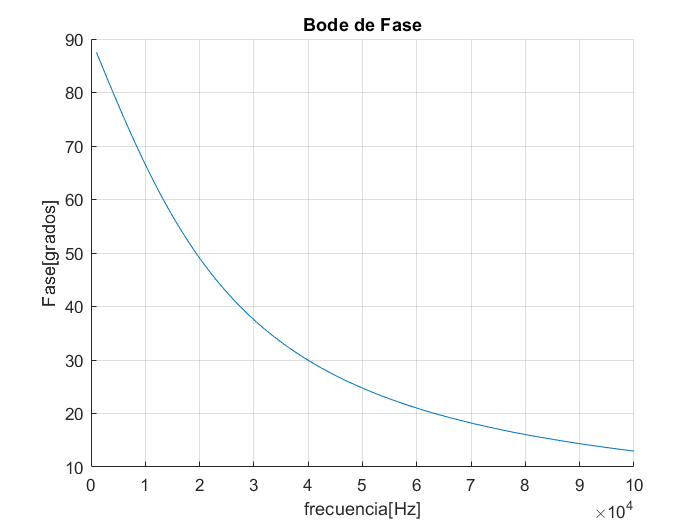
\includegraphics[scale=0.5]{2teofase.png}
\caption{Diagrama de Bode Teorico.}
\label{fig:CR}
\end{figure}

\subsection{Tabla de Mediciones}

Exitando el circuito con una onda senoidal de $10~V_{pp}$, obtuvimos los siguientes resultados:

\begin{table}[!htb]
\centering
\begin{tabular}{|c|c|c|c|c|}
\hline
f{[}Hz{]}    & $|V_{in}|${[}V{]} & $|V_R|${[}V{]}      & $H(s)=\frac{V_R}{V_{in}} (s)${[}dB{]} & $\phi${[}grados{]} \\ \hline
1.00E+03  & 10    & 4.80E-01 & -26.6           & 90                  \\ \hline
5.00E+03  & 10    & 2.28     & -12.9           & 78.52165905         \\ \hline
1.00E+04  & 10    & 4.15     & -7.6            & 63.75353139         \\ \hline
1.50E+04  & 10    & 5.55     & -5.1            & 52.27906148         \\ \hline
1.70E+04  & 10    & 6        & -4.4            & 49.46419789         \\ \hline
2.00E+04  & 10    & 6.5      & -3.7            & 45.15361072         \\ \hline
2.05E+04  & 10    & 6.6      & -3.6            & 44.26676315         \\ \hline
2.10E+04  & 10    & 6.67     & -3.5            & 43.86805655         \\ \hline
2.13E+04  & 10    & 6.7      & -3.4            & 43.07852077         \\ \hline
2.16E+04  & 10    & 6.75     & -3.4            & 42.76554885         \\ \hline
2.19E+04  & 10    & 6.8      & -3.3            & 37.66184465         \\ \hline
2.24E+04  & 10    & 6.87     & -3.2            & 41.66698377         \\ \hline
2.28E+04  & 10    & 6.96     & -3.1            & 41.59799164         \\ \hline
2.30E+04  & 10    & 7        & -3.1            & 40.91964995         \\ \hline
2.32E+04  & 10    & 7.02     & -3              & 40.54160187         \\ \hline
2.34E+04  & 10    & 7.05     & -3              & 40.39097962         \\ \hline
2.38E+04  & 10    & 7.1      & -3              & 40.07576311         \\ \hline
2.40E+04  & 10    & 7.12     & -2.9            & 39.92617229         \\ \hline
2.45E+04  & 10    & 7.2      & -2.8            & 39.03536844         \\ \hline
2.50E+04  & 10    & 7.24     & -2.8            & 38.82913316         \\ \hline
2.80E+04  & 10    & 7.54     & -2.4            & 35.80299001         \\ \hline
3.00E+04  & 10    & 7.72     & -2.2            & 33.43564423         \\ \hline
3.50E+04  & 10    & 8.04     & -1.8            & 29.86776904         \\ \hline
4.00E+04  & 10    & 8.3      & -1.6            & 27.06493423         \\ \hline
4.50E+04  & 10    & 8.5      & -1.4            & 24.88510514         \\ \hline
5.00E+04  & 10    & 8.64     & -1.2            & 21.14319164         \\ \hline
5.50E+04  & 10    & 8.75     & -1.1            & 20.48731511         \\ \hline
6.50E+04  & 10    & 8.9      & -1              & 17.18152467         \\ \hline
7.50E+04  & 10    & 9        & -9.00E-01       & 15.96201416         \\ \hline
8.00E+04  & 10    & 9.06     & -8.00E-01       & 13.85703185         \\ \hline
8.50E+04  & 10    & 9.1      & -8.00E-01       & 12.55578123         \\ \hline
\end{tabular}
\caption{Modulo de Tensiones, Magnitud y Fase de la funcion de transferencia.}
\end{table}

\subsection{Analisis de Resultado}

Con el uso de los datos hallados en el punto anterior conseguimos los siguientes diagramas, los cuales se superpuso la tension de $V_R$, $\frac{V_R}{V_{in}}$ y los valores teoricos de la funcion de transferencia. 

\begin{figure}[h!]
\centering
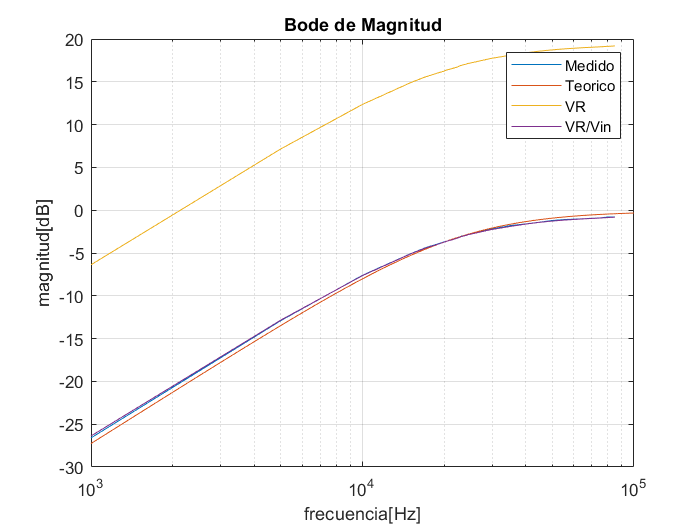
\includegraphics[scale=0.5]{2Compmag.png}
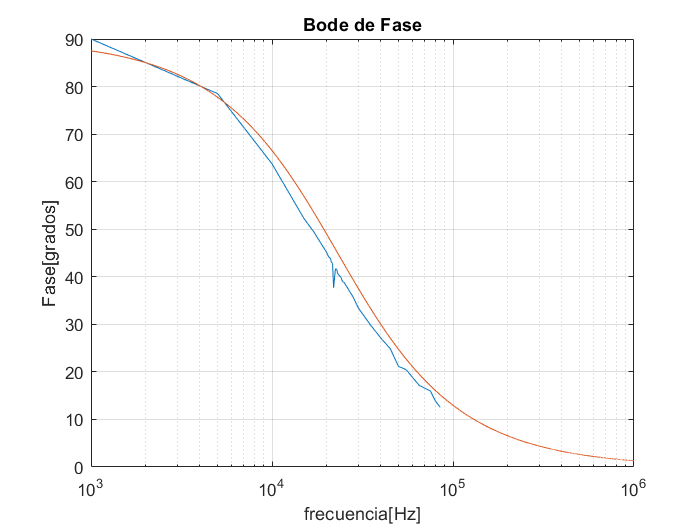
\includegraphics[scale=0.5]{2Compfase.png}
\caption{Diagramas de Amplitud y Frecuencia del circuito CR.}
\label{fig:CR}
\end{figure}

En la figura notamos una leve distincion entre los valores de amplitud y frecuencia de los medidos y los teoricos; esto se debe a que pudo haber errores accidentales durante medicion y ademas los componentes no son perfectos, por lo que presentan impedancia parásita causando alteraciones impredecibles durante la medicion. Pero es posible la identificacion del circuito CR como un filtro pasa altos.
En la grafica el $V_R$ no es  



>>>>>>> 90e60842c18f4bfcd674f06bb288a364d338db0a

\section{Respuesta en frecuencia con barrido automático}

\subsection{Modo normal del osciloscopio}

El barrido automático se realizó con el generador en donde se barrió
de 100Hz a 2MHz en un lapso de 100 mili segundos con una senoidal
de 20 $V_{pp}$. El output del generador se utilizó para excitar al
circuito RC y se conectó el sync al osciloscopio para poder triggerear
la señal, además se aprovechó el marker del sweep del generador para
que la cuadrada entregada por el sync tenga un ancho de 22,6KHz para
que coincida con la frecuencia de corte calculada de nuestro circuito.
Cabe mencionar que el barrido automático estaba configurado en escala
logaritmica. Se obtuvó la siguiente imagen:

\begin{figure}[H]
\begin{center}
%\includegraphics[bb = 0 0 200 100, draft, type=eps]{./Respuesta en frecuencia barrido automatico modo normal.png}
\par\end{center}
\caption{Respuesta en frecuencia con barrido automatico en modo normal}
\end{figure}

La figura evidencia claramente el efecto del filtro pasa bajos sobre
el circuito, mientras que la señal amarilla que es la entrada se
mantiene constante en amplitud a lo largo de todo el barrido, la salida
que es la senial verde tiene ganancia unitaria en las bajas frecuencias
y luego se atenua a medida que esta aumenta. La senial cuadrada violeta
marca la frecuencia de corte del circuito donde se espera una caida
de 3dB. En veces equivale aproximadamente a una atenuacion de $\sqrt{2},$es
decir, $V_{0}=\sqrt{2}V_{i}$ y en nuestro caso como $V_{i}$ tiene
una amplitud de 10 V, $V_{0}$ deberia tener una amplitud aproximada
de 7,1 V, esto se puede observar claramente en el gráfico.

\subsection{Modo XY del osciloscopio}

Se intento de siumular el barrido en el modo XY bajo ciertas características.
Se colocó un generador realizando un sweep barriendo nuevamente frecuencias
de $100Hz$ a $2MHz$ esta vez linieal cada $10ms$ con una senoidal
$20Vpp$ y bajo estas condiciones se lo conectó a la entrada del circuito.
Luego se sincronizó el trigger del generador de sweep con el flanco
descendente de la señal del generador 2, en el cual se colocó una
rampa de $10Vp$ a una periodo de $11ms$ y se la conectó en la entrada
X del osciloscopio. Se conectó la salida del circuito a la entrada
Y del osciloscopio. Por consecuente, tomando en cuenta las consideraciones
establecidas, se esperaba ver como en el modo XY el eje Y iba a presentar
las senoidales en modo sweep desde la frecuencia inicial a la final
y en la componente X un desplazamiento de 0 a 10V estableciendo la
relación $0V$ a $t=\text{0}$ y en $10V$ $t=11ms$ dejando entrar
un poco mas de un barrido en pantalla.
\begin{figure}[H]
\centering{}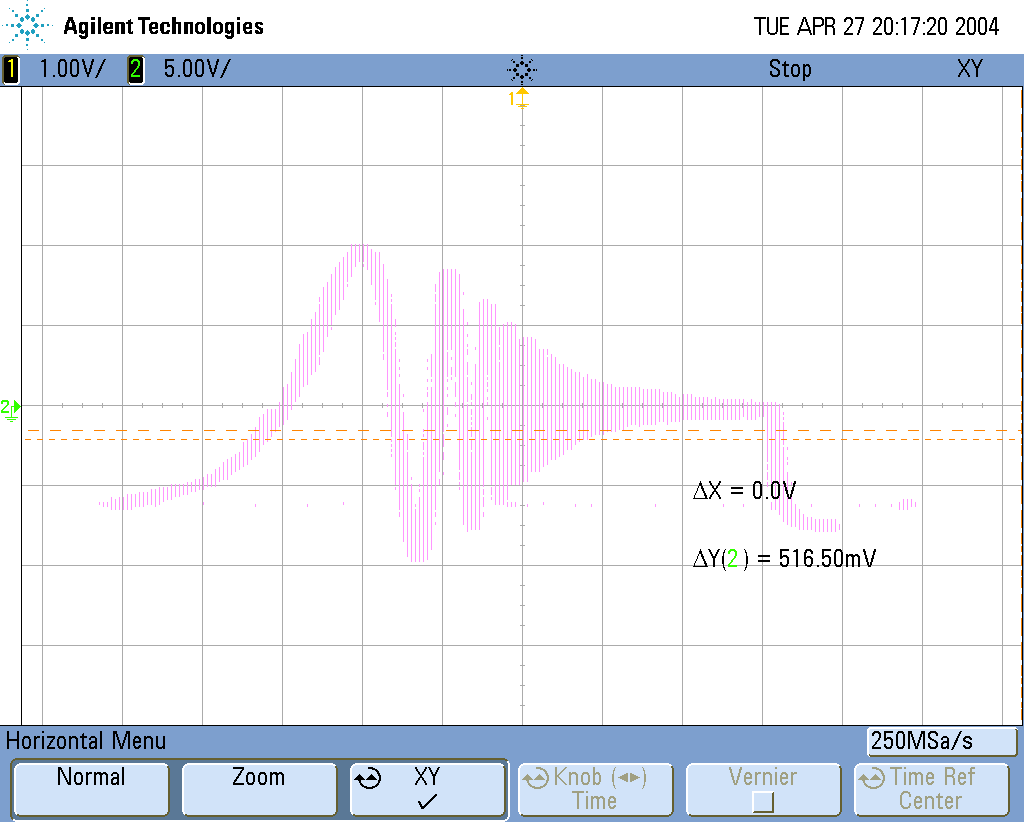
\includegraphics{./scope_24.png}\caption{Respuesta en frecuencia con barrido automático en modo XY}
\end{figure}

Se puede observar como las configuraciones previas permitieron el
análisis en frecuencia del circuito, dando una imagen relacionada
directamente con la obtenida en el modo normal del osciloscopio bajo
el mismo sweep. Es importante notar como se configuró la escala en
X y en Y para poder formar correctamente la imagen en pantalla del
barrido en frecuencia.

\section{Respuesta en frecuencia del osciloscopio}

Para medir la respuesta en frecuencia del osciloscopio se utilizaron
dos puntas de osciloscopio y un generador, por un lado se conectaron
ambas puntas con el generador de seniales entre sí y por el otro las
masas de estos tres elementos también entre sí. El bode del circuito
se realizó con los filtros AC y el BW del osciloscopio activados y
se lo excitó con una senoidal de 10 $V_{pp}$. Los resultados obtenidos
de las mediciones se graficaron en la siguiente figura:
\begin{figure}[H]
\caption{Respuesta en frecuencia del osciloscopio}
\end{figure}

Se puede observar que la forma de la respuesta en frecuencia es la
de un filtro pasa banda ya que atenua las frecuencias menores a 12Hz
y las frecuencias mayores a 5MHz. Esto se debe a que el filtro AC
del osciloscopio filtra las seniales continuas con un capacitor formando
un pasa altos que posee una frecuencia de corte muy pequenia; y el
filtro BW dismunuye el ancho de banda atenuando las altas frecuancias
mediante un filtro pasa bajo, la combinación de ambos actuan como
el pasa banda representado en la figura 1.
\end{document}
